\documentclass{beamer}

%%%%%% Packages %%%%%
%\usepackage{scrpage2}
%\usepackage{amssymb}
%\usepackage{amsmath}
\usepackage[style=authoryear,backend=biber]{biblatex}
%\usepackage[flushmargin,ragged]{footmisc}
% \usepackage{graphicx}
%\usepackage{ifthen}
% \usepackage{lastpage}
%\usepackage{ngerman}
\usepackage{calc}
\usepackage{enumerate}
\usepackage{nag}
% \usepackage{hhline}
%\usepackage{listings}
%\usepackage{xr-hyper}
\usepackage{hyperref}
%\usepackage{siunitx}
\usepackage{tikz}
% \usepackage{xcolor}
\usepackage{xltxtra}

\addbibresource{../report/references.bib}

\usetikzlibrary{arrows, calc, chains}

\usecolortheme{beaver}
\defaultfontfeatures{Mapping=tex-text}
\setsansfont{Helvetica Neue}

\useinnertheme{rounded}
\setbeamertemplate{itemize items}[circle]
\setbeamertemplate{navigation symbols}{}
\setbeamertemplate{footline}[frame number]
\setbeamertemplate{blocks}[rounded][shadow=true]
\setbeamercolor{block title}{bg=frametitle.bg}
\setbeamercolor{block body}{bg=frametitle.bg}
\setbeamercolor{block title alerted}{bg=frametitle.bg}
\setbeamercolor{block body alerted}{bg=frametitle.bg}
\renewcommand*{\bibfont}{\scriptsize}

%%%%% Eigene Format-Kommandos %%%%%
\newcommand{\credit}[2]{ %
    \begin{tikzpicture} %
        \tikzstyle{every node}=[inner sep=0] %
        \node  (img) {#1}; %
        \node [below=0 of img.south west, anchor=north west] {\tiny #2}; %
    \end{tikzpicture}}

%%%%% Externe Dokumente %%%%%

%%%%% Silbentrennung %%%%%

%%%%% Weiteres %%%%%
%\lstset{basicstyle=\fontfamily{pcr}\selectfont, keywordstyle=\bfseries, language=C++}

\title{Effects of Inhibitory Synaptic Scaling on the Balance of Excitation and 
    Inhibition}
\subtitle{Lab rotation supervised by Henning Sprekeler}
\author{Jan Gosmann}
\date{May 15, 2013}
\hypersetup{
  pdftitle={\@title},
  pdfauthor={\@author},
  pdfsubject={},
  pdfkeywords={}
}

\begin{document}
\maketitle

\begin{frame} \frametitle{Inhibition-excitation balance}
    \begin{center}
        \credit{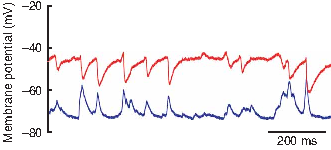
\includegraphics[width=\textwidth]{figures/iebalance}}{\textcite{Okun:2008db}}
    \end{center}
\end{frame}

\begin{frame} \frametitle{Feedforward inhibition}
    \begin{center}
        \credit{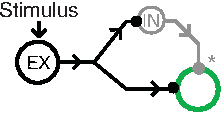
\includegraphics[width=0.6\textwidth]{../report/figures/ff_inhibition}}{\textcite{Vogels:2011wr}}
    \end{center}
    \pause
    \structure{Inhibitory plasticity}
    \begin{equation*}
        \Delta w = \eta(\text{pre} \times \text{post} - \rho_0 \times 
        \text{pre})
    \end{equation*}
\end{frame}

\begin{frame} \frametitle{Before learning}
    \begin{center}
        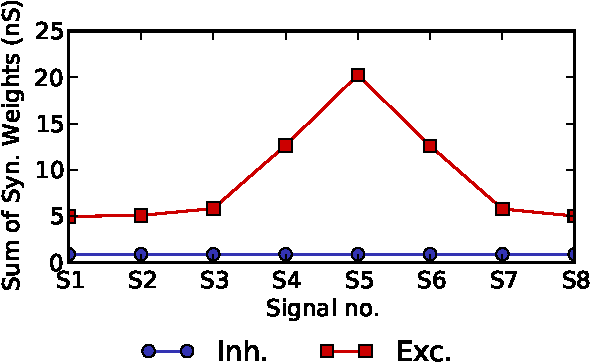
\includegraphics[width=\textwidth]{figures/weights_before}
    \end{center}
\end{frame}

\begin{frame} \frametitle{After learning}
    \begin{center}
        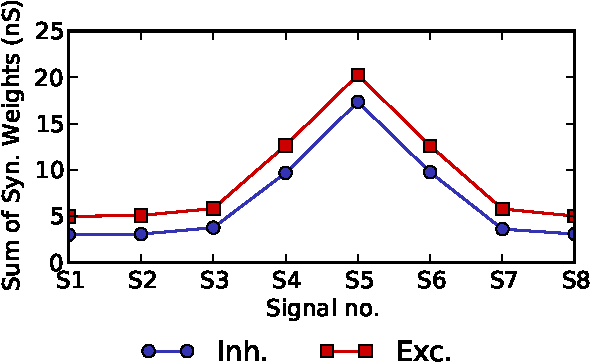
\includegraphics[width=\textwidth]{figures/weights_after}
    \end{center}
\end{frame}

\begin{frame} \frametitle{Time Evolution of Firing Rate and Weights}
    \begin{center}
        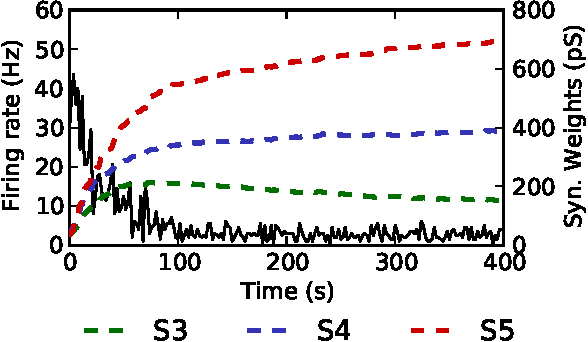
\includegraphics[width=\textwidth]{figures/evo_orig}
    \end{center}
\end{frame}

\begin{frame} \frametitle{Modified Learning Rule}
    \begin{equation*}
        \Delta w = \eta(\text{pre} \times \text{post})
        \quad\text{and}\quad
        \tau_w \frac{dw}{dt} = -\eta w
    \end{equation*}
    \begin{center}
        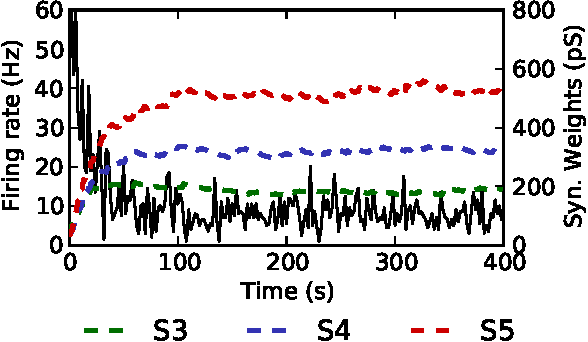
\includegraphics[width=\textwidth]{figures/evo_exp_decay}
    \end{center}
\end{frame}

\begin{frame} \frametitle{Firing Rates}
    \begin{center}
        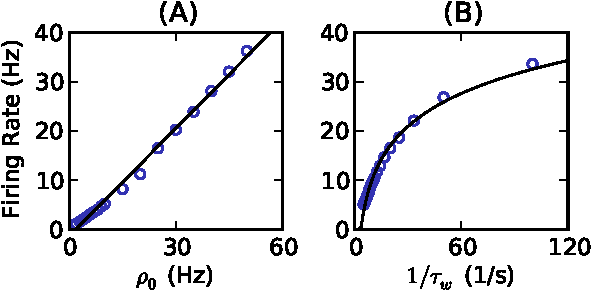
\includegraphics[width=\textwidth]{figures/rates}
    \end{center}
\end{frame}

\begin{frame} \frametitle{Response Properties}
    \begin{center}
        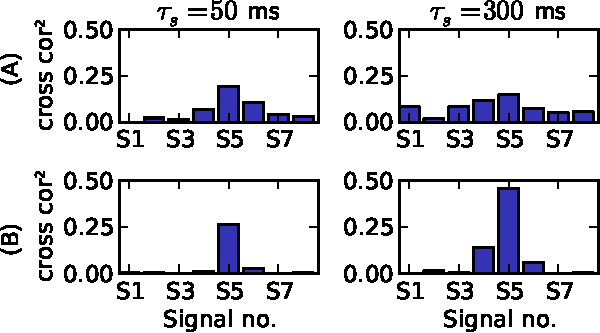
\includegraphics[width=\textwidth]{figures/correlations}
    \end{center}
\end{frame}

\begin{frame} \frametitle{Excitatory Plasticity}
    \begin{center}
        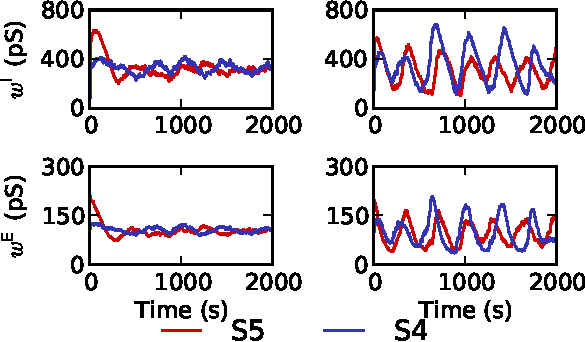
\includegraphics[width=\textwidth]{figures/exc-stdp-mult-l2}
    \end{center}
\end{frame}

\begin{frame} \frametitle{Summary}
    \begin{itemize}
        \item Different learning rules achieve balance of inhibition and 
            excitation.
        \item Detailed neuron behavior can differ despite balance.
        \item Exponential decay allows balance while retaining stimulus tuning.
        \item Excitatory plasticity can lead to oscillations.
        \item Excitatory plasticity can destroy stimulus tuning.
    \end{itemize}
\end{frame}

\begin{frame} \frametitle{Thank you for your attention!}
    \printbibliography
\end{frame}

\end{document}
